  %# -*- coding: utf-8-unix -*-
%%==================================================
%% chapter03.tex for SJRU Master Rhesis
%% related work
%%==================================================
%\bibliographystyle{sjtu2}%[此处用于每章都生产参考文献]

% equation有编号 displaymath无编号

\theoremstyle{definition}
\newtheorem{definition}{定义}[section]

\chapter{相似轨迹查询方法实现}
\label{chap:implementation}

\section{k最佳连接}
\label{sec:k-bct}
一个轨迹数据库中存储了大量的原始车载GPS轨迹或是已经预处理过的车载GPS轨迹。这里的轨迹由一系列的地理位置点组成$\{p_{1},p_{2},p_{3},\cdots, p_{m}\}$,其中$p_{i}$ $1\leq i \leq m$代表一个由经度和维度构成的地理位置点而$m$代表轨迹中点的数目。本文所定义的k最佳连接查询(k Best-Connected Rrajectory Query)的输入由一组查询点$Q$组成。$q_{j}$ $1 \leq j \leq n$和$p_{i}$定义相同,其中n是查询点的数目。这里用户可以选择选择是否在查询中指定轨迹连接依照查询点的先后顺序,即是否选择查询有序性。若选择查询有序性,则查询点集$Q$为认为是从$q_{1}$到$q_{m}$有序点集。
\begin{displaymath}
	Q = \{q_{1},q_{2},q_{3},\cdots, q_{n}\}
\end{displaymath}

在搜索最好连接轨迹这一上下文中,相似度方程的定义需要和传统方法有所不同,在这里我们将相似度方程定义为一条轨迹连接查询点的好坏程度。因此,本文首要考虑一条轨迹到每一个查询点的距离,我们简要定义距离一个查询点$q_{i}$到一条轨迹$R=\{p_{1},p_{2},p_{3},\cdots, p_{m}\}$的距离为$D_{q}$,即

\begin{equation}
	\label{eq3-1}
	D_{q}(q_{i}, R) = \min_{p_{j} \in R} \{D_{e}(q_{i}, p_{j})\} 
\end{equation}

式\ref{eq3-1}中,$D_{e}(q_{i}, p_{j})$是指查询点$q_{i}$和轨迹点$p_{j}$之间的欧氏距离,因此通常意义上相似度距离$D_{q}$代表从查询点$q_{i}$到轨迹上任一一点距离的最短距离。当我们找到轨迹上一点$p_{j}$是离查询点$q_{i}$的最短距离点时,我们将$<q_{i},p_{j}>$作为最短匹配点对。在无序查询点击中,我们定义查询点集$Q$和轨迹$R$之间的相似度为$Sim(Q,R)$。

\theoremstyle{definition}
\begin{definition}
	轨迹$R={p_{1}, p_{2}, \cdots, p_{n}}$而查询点为$q$,$<q, p_{i}>$表示一组匹配点对。对于$\forall p_{i} \neq p_{j}$, $d_{e}(p_{i}, q)\leq d_{e}(p_{j}, q)$,那么$<p_{i}, q>$是轨迹$R$到查询点$q$的最短匹配点对。
\end{definition}

\begin{equation}
	\label{eq3-2}
	Sim(Q,R) = \sum_{i=1}^{n} \emph{e}^{-D_{q}(q_{i}, R)}
\end{equation}

式\ref{eq3-2}将每个查询点对$Sim(Q,R)$的贡献值通过自然对数去反得以体现,即根据自然函数的单调性,查询点离轨迹越近,则$-D_{q}(q_{i}, R)$越大,以自然对数为底取幂的值也越大,最后使得$Sim(Q,R)$的值也越大。从用户人为角度和地理语义角度上看,一条轨迹与所有的查询点被定义为相似当且仅当这条轨迹和所有的查询点都十分接近。

图\ref{fig:3-1}通过距离说明查询点和轨迹之间的匹配关系。如图\ref{fig:3-1}(a)所示,查询点$q_{1}$、$q_{2}$和$q_{3}$分别与轨迹R上的轨迹点$p_{6}$、$p_{4}$和$p_{7}$最近匹配,根据式\ref{eq3-2}可以得出,$Sim(Q,R) = \emph{e}^{-D_{q}(q_{1}, p_{6})} + \emph{e}^{-D_{q}(q_{2}, p_{4})} + \emph{e}^{-D_{q}(q_{3}, p_{7})} = \emph{e}^{-1.5}+ \emph{e}^{-0.1} + \emph{e}^{-0.1}$。

另一方面,选择查询点和轨迹之前进行有序查询时,顺序性是需要在查询过程中予以考虑。对于查询点$q_{i}$而言,最近匹配点或许并不在是距离上最近的轨迹点$p_{j}$。因此,相似度方程在此步骤中应该适当调整。我们再借用图\ref{fig:3-1}予以说明。假设以下用户场景:用户希望查询出一条以$q_{1} \rightarrow q_{2} \rightarrow q_{3}$为顺序的相似轨迹,显然图\ref{fig:3-1}(a)中的顺序并不再符合用户需求。实际的有序查询结果顺序如图\ref{fig:3-1}(b)是$p_{3} \rightarrow q_{4} \rightarrow q_{7}$。在考虑有序性的相似查询规程中,我们的目标是在保持查询有序性的同时追求每一对匹配点对相似度的最大贡献值,即从图\ref{fig:3-1}(b)可以看出$<q_{1},p_{3}>, <q_{2},p_{4}>, <q_{3},p_{7}>$这样的三对匹配点是所有有序匹配对中使得相似度最大的情况。

\begin{figure}[!htp]
  \centering
  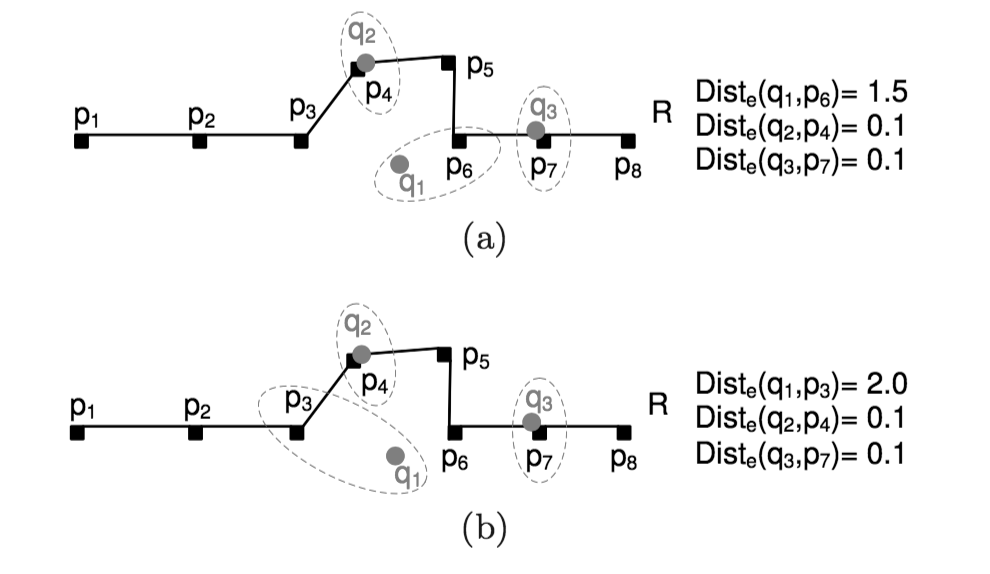
\includegraphics[width=0.7\textwidth]{chapter03/similarity.png}
  \bicaption[fig:3-1]{这里将出现在插图索引中}{查询点与轨迹之间的匹配}{Fig}{Match between query points and trajectory}
\end{figure}

有序查询的相似性计算和无序查询也有区别。给定一组有序的查询点$Q_{o} = \{q_{o1},q_{o2},q_{o3},\cdots, q_{on}\}$和一条已有轨迹$R$,我们通过递归思想为有序查询重新定义相似度方程为$Sim_{o}(Q,R)$,式\ref{eq3-3}。其中$Head(x)$函数代表$x$中的第一个点,例如$Head(Q)$是查询点$q_{1}$;同时$Rest(x)$表示$x$去掉x第一个点之后剩余的部分,例如$Rest(Q)$代表\{$q_{2},q_{3},\cdots, q_{n}$\}。在式\ref{eq3-3}中,通过递归的想法,本文将对$Sim_{o}(Q,R)$的求最大值问题分为对两个子问题的求解,即分别计算$Sim_{o}(Rest(Q),R)$和$Sim_{o}(Q,Rest(R))$的最大值问题。当$Head(Q)$和$Head(R)$的两个轨迹点匹配的时候,我们可以将$e^{-D_{e}(Head(Q), Head(R))}$提前计算并加入当后面计算的$Sim_{o}(Rest(Q),R)$之中。在这种情况下,$Head(R)$需要为下一轮的比较计算继续保留,因为对于$Rest(Q)$中的查询点来说,$Head(R)$依旧有可能成为最佳匹配点。而当当$Head(Q)$和$Head(R)$不匹配的时候时我们则跳过$Head(R)$计算$Sim_{o}(Q,Rest(R))$。这种求解思路类似于动态规划的思路,这也为我们再后面优化过程中通过动态规划的来解决这一问题提供了参考。式\ref{eq3-3}结合了动态时间规整(DTW)利用重复点和最长公共子序列(LCSS)省略不匹配点的优点来计算相似度方程。

\begin{equation} 
\label{eq3-3} 
Sim_{o}(Q,R)= max \left\{  
	\begin{array}{lr}  
    e^{-D_{e}(Head(Q), Head(R))} + Sim_{o}(Rest(Q),R) & \\
    Sim_{o}(Q,Rest(R)) &  
    \end{array}  
\right.  
\end{equation}  

根据相似度方程,本文可以对k最佳连接查询有以下定义3.1.2.:

%\begin{thm}[k最佳连接]
%	给定一组轨迹集合 $T = {R_{1}, R_{2}, R_{3} \cdots, R_{n}}$、一组查询点$Q = {q_{1},q_{2},q_{3},\cdots, q_{n}}$和对应的相似度方程$Sim$,k最佳连接查询则可以从轨迹集合$T$中找到k条轨迹$T'$,满足式\ref{eq3-4}:
%	\begin{equation}
%		\label{eq3-4}
%		Sim(Q,R_{i})_{R_{i} \in T'} \geq Sim(Q,R_{j})_{R_{j} \in T-T'}
%	\end{equation}
%	其中$Sim$根据用户定义选择是否考虑有序性。
%\end{thm}

\theoremstyle{definition}
\begin{definition}
	给定一组轨迹集合 $T = {R_{1}, R_{2}, R_{3} \cdots, R_{n}}$、一组查询点$Q = {q_{1},q_{2},q_{3},\cdots, q_{n}}$和对应的相似度方程$Sim$,k最佳连接查询则可以从轨迹集合$T$中找到k条轨迹$T'$,满足式\ref{eq3-4}。其中$Sim$根据用户定义选择是否考虑有序性。:
	\begin{equation}
		\label{eq3-4}
		Sim(Q,R_{i})_{R_{i} \in T'} \geq Sim(Q,R_{j})_{R_{j} \in T-T'}
	\end{equation}
\end{definition}

\section{相似轨迹查询处理过程}
\label{sec:query processing}

\subsection{问题概述}
\label{sec:problem Forumation}
轨迹数据为一组有序点集,轨迹$R$可以被表示为$R={p_{1}, p_{2}, \cdots, p_{n}}$,其中$p_{i}$是轨迹$R$的在时间顺序上的第$i$个轨迹点。对于本文应用而言,查询点集$Q$被定义为一组点集$Q={q_{1}, q_{2}, \cdots, q_{m}}$,且根据具体情况定义是否有序。在根据上文设计的相似性距离和k最佳连接定义后,我们将我们相似轨迹查询任务等价转化为k最佳连接查询,并产生下面的定义:

\theoremstyle{definition}
\begin{definition}
	给定已有的轨迹数据集$D$,和一条待查询轨迹$R_{q}$。我们通过轨迹简化算法\ref{algo:ts}将待查询轨迹$R_{q}$转换成一组查询点集$Q$。通过k最佳连接查询方法,从轨迹数据集$D$中获取k条轨迹,集合为$D' = {R_{1}, R_{2}, \cdots, R_{k}}$,满足式\ref{eq3-5}。其中$Sim$根据用户定义选择是否考虑有序性。:
	\begin{equation}
		\label{eq3-5}
		Sim(Q,R_{i})_{R_{i} \in D'} \geq Sim(Q,R_{j})_{R_{j} \in D-D'}
	\end{equation}
	我们称$D'$轨迹数据集合为对于轨迹$R_{q}$的k条最相似轨迹查询结果。
\end{definition}

处理上述问题的直观方法可以选择对轨迹集合$D$进行全局搜索,维护一个关键字为相似度大小的优先队列,然后返回结果。但对于系统而言,这样处理数据过于浪费时间。

为解决上述问题,我们首先需要明确我们查询输入的优势在于我们输入的查询点相对于传统的相似轨迹查询方法要小。这是我们能够合理且有效运用空间索引分别对每一个查询点应用近邻查询,并合并查询结果生成k最佳相似轨迹的基本前提。这一方法的搜索复杂度相对于查询点集来说相对恒定。因此,当得出一条轨迹对于查询点集的最近轨迹点便为我们计算该条轨迹与查询点集相似度的上下界提供可能。本文中使用R树索引并搜索近邻的轨迹点,当我们找到关于某个查询点$q$的最近轨迹点$p$,那么包含$p$轨迹点的轨迹一定是离该查询点$q$最近的一条轨迹。

其次在设计搜索框架过程中,我们借鉴\emph{备选和筛选}(candidate generation and refinement)这一思路。这一思路最初提出为在分布式系统中进行k最大数据处理。首先每个子系统的数据按从大到小排列然后并行合并后进行筛选,选出最好的k个结果。这一思路结合k最近邻查询符合本文对算法设计的要求,我们对查询点集$Q$中的每一个点都进行查询并将他们的结果合并生成暂时的轨迹备选集,然后通过筛选的方法选出最相似的k条轨迹。问题的关键在于如何进行轨迹备选集的搜索,以及如何保证k条最相似轨迹的完备性。

本文的相似轨迹查询方法利用R树数据结构,通过简单的k最近邻算法并在其基础上进行有效深度拓展和具体实践优化实现k最佳连接查询以实现相似轨迹查询。表\ref{tab-notations}提供了本文需要的基本符号及其注释。
\\
\begin{table}[!htpb]
  	\centering
		\begin{tabular}{ |p{3cm}||p{9cm}|  }
		\hline
		符号标记 & 符号注释 \\
		\hline
		$N$ & 一条轨迹的轨迹点总数目 \\
		\hline
		$m$ & 一组查询点总数目 \\
		\hline
		$D_{e}(q_{i},p_{j})$ & 点$q_{i}$和点$p_{j}$之间的欧氏距离 \\
		\hline
		$D_{e}(q_{i},p_{j})$ & 点$q_{i}$和点$p_{j}$之间的欧氏距离 \\
		\hline
		$D_{q}(q_{i},R)$ & 点$q_{i}$和轨迹$R$之间的最短距离 \\
		\hline
		$C$ & 轨迹备选集 \\
		\hline
		$\epsilon$ & TBD\\
		\hline
		$r$ & $\lambda$-NeareatNeighbor搜索半径\\
		\hline
		$\rho$ & 轨迹点密度\\
		\hline
		$\xi$ & 查询点$q_{i}$对相似度上界贡献度\\
		\hline
		$\mu,\upsilon$ & 优化搜索权值\\
		\hline
		\end{tabular}
	\bicaption[tab-notations]{出现在表目录的标题}{本文符号列表及其对应注释}{Table}{A list of notations and explanations}
\end{table}
\\

\subsection{生成轨迹备选集}
\label{subsec:candidate-generation}
将预处理的轨迹点存储在R树之中后,我们可以有效地通过k最近邻搜索方法来找到离某一查询点$q$最近的一条轨迹。假设现有一组查询点$Q = \{q_{1},q_{2},\cdots, q_{m}\}$,进行无序的相似轨迹查询。我们首先对这一组查询点中的每一个查询点进行$\lambda NN$查询并得到结果如下:

\begin{align*}
\lambda NN(q_{1}) &= \{p_{1}^{1}, p_{1}^{2}, p_{1}^{3}, \cdots, p_{1}^{\lambda}\}\\ 
\lambda NN(q_{2}) &= \{p_{2}^{1}, p_{2}^{2}, p_{2}^{3}, \cdots, p_{2}^{\lambda}\}\\ 
\cdots\\
\lambda NN(q_{m}) &= \{p_{m}^{1}, p_{m}^{2}, p_{m}^{3}, \cdots, p_{m}^{\lambda}\}
\end{align*}

通过每个查询点根据$\lambda NN$算法生成的结果,我们根据结果中的点生成我们的轨迹备选集。包含$\lambda NN(q_{i})$中至少一个轨迹点的轨迹被加入到轨迹备选子集$C_{i}$中用于之后生成k最佳连接结果。在这一步我们需要保证轨迹备选子集$C_{i}$的基数应该小于等于$\lambda$,因为多个属于$\lambda NN(q_{i})$的轨迹点有可能属于同一条轨迹。之后我们合并所有由$\lambda NN(q_{i})$查询结果得出的轨迹备选子集以获取一个包含$f$条轨迹的轨迹备选集$C$

\begin{equation} 
 C = \bigcup_{i=1}^{m} C_{i} = \{R_{1}, R_{2}, \cdots, R_{f}\} \nonumber
\end{equation}  

对于轨迹备选集$C$中的每一条轨迹$R_{x} (1 \leq x \leq f)$而言,$R_{x}$必须包含至少一个离对应查询点距离在固定范围内的轨迹点。即假使$R_{x}$属于某一轨迹备选子集$C_{i}$($C_{i}$为轨迹备选集$C$的子集),那么$\lambda NN(q_{i})$中的应该包含轨迹$R_{x}$上的一点且$q_{i}$到轨迹$R_{x}$的最短距离是已经计算过的。由于轨迹$R_{x}$和查询点$q_{i}$至少有一组已知的匹配点,则我们可以通过已知匹配点来计算出轨迹备选集中轨迹与查询点集相似度的下界,我们定义为$LB$(lower bound)。

\begin{equation}
	\label{eq3-6}
	LB(R_{x}) = \sum_{1\leq i\leq m \wedge R_{x}\in C_{i}}\bigg( \max_{1\leq j\leq \lambda \wedge p_{i}^{j}\in R_{x}}e^{-D_{e}(q_{i}, p_{i}^{j})}\bigg)
\end{equation}


在计算下界的时候,我们考虑的查询点集为$Q_{matched}$ = \{$q_{i} | 1\leq i\leq m \wedge R_{x} \in C_{i}$\},对于$Q_{matched}$中的查询点来说,他们和轨迹$R_{x}$上的某一个轨迹点在进行k最近邻查询中被计算作为匹配点,即对于查询点$q_{i} \in Q_{matched}$,我们可以找到轨迹上的某一点$p_{i}^{j}$满足$e^{-D_{e}(q_{i}, p_{i}^{j})}$达到最大值,因为在欧氏距离上$q_{i}$与$p_{i}^{j}$最为接近,根据这一点我们可以将式\ref{eq3-6}中的$\max_{1\leq j\leq \lambda \wedge p_{i}^{j}\in R_{x}}e^{-D_{e}(q_{i}, p_{i}^{j})}$等价写成$e_{-D_{q}(q_{i}, R_{x})}$,得出式\ref{eq3-7}

\begin{equation}
	\label{eq3-7}
	LB(R_{x}) = \sum_{1\leq i\leq m \wedge R_{x}\in C_{i}}e^{-D_{q}(q_{i}, R_{x})}
\end{equation} 

显然这个相似度下界值不会大于$\sum_{i=1}^{m} e^{-D_{q}(q_{i}, R(x))}$,因为在计算相似度下界的时候值考虑了与在轨迹$R_{x}$上与某些查询点匹配轨迹点。另一方面,加入轨迹$R_{x}$不属于某个备选轨迹子集$C_{i}$,则轨迹$R_{x}$上任意轨迹点都不会存在于由查询点$q_{i}$得到的k最近邻查询结果$\lambda NN$中。这说明由式\ref{eq3-6}或\ref{eq3-7}定义的相似度下界计算对于式\ref{eq3-2}是成立的。

对于在不属于轨迹备选集$C$中的轨迹($R_{ns} \notin C$),这些轨迹并没有在查询点集进行k最近邻查询中被扫描,他们到查询点$q_{i}$的距离将会小于$p_{i}^{\lambda}$到查询点$q_{i}$的最短距离,即$D_{e}(q_{i}, p_{i}^{\lambda})$。这一发现能让我们计算出所有不属于轨迹备选集的轨迹$R_{ns}$对于查询点集的相似度的上界,我们定义为定义为$UB_{ns}$(upper bound)。

\begin{equation}
	\label{eq3-8}
	UB_{ns} = \sum_{i=1}^{m}e^{-D_{e}(q_{i}, p_{i}^{\lambda})}
\end{equation}

当我们在进行有关空间意义上的数据搜索的时候,剪枝是保证搜索效率的重要手段。相似度的上下界让我们可以设计出针对k最佳连接的剪枝算法以限制搜索空间,提高搜索效率,避免了对整个轨迹数据集或者对不满足条件的轨迹进行多余操作。根据相似度的上下界我们提出下述定理:
\\

\begin{thm}[相似度上下界]
	\label{thm3-1}
	假设对于相似轨迹插叙的k最佳连接算法没有有序性限制,我们可以在对查询点集进行一轮k最近邻查询(k=$\lambda$)之后的轨迹备选集C中,选取一个包含k条轨迹的一个轨迹子集$C'$。当$\min_{R_{x}\in C'}{LB(R_{x})}\geq UB_{us}$这一条件满足时,我们可以从轨迹备选集$C$中获得k条最佳连接轨迹,即k条与查询点集最相似的轨迹。
	\begin{proof}
	首先对于轨迹子集$C'$中的某一条轨迹$R_{a}$($R_{a} \in C'$)而言,轨迹$R_{a}$满足$Sim(Q,R_{a}) \geq LB(R_{a})$。与此同事,对于轨迹备选集$C$之外的轨迹$R_{b}$($R_{b} \notin C$),轨迹$R_{b}$满足$UB_{ns} \geq Sim(Q,R_{b})$。当上述定理成立时,即$\min_{R_{a}\in C'}{LB(R_{a})}\geq UB_{ns}$,我们可以推断出$\forall R_{a}\forall R_{b} \big( R_{a} \in C' \wedge R_{b} \notin C \big)$,$Sim(Q,R_{a}) \geq Sim(Q,R_{b})$成立。这也证明了对于查询点集$Q$得到的k最佳连接的结果轨迹在这个时候应该全部在轨迹备选集$C$中。
	\end{proof}
\end{thm}

需要注意的是定理\ref{thm3-1}中的轨迹子集$C'$不一定全是k最佳连接轨迹的结果,我们只能保证k最佳连接的轨迹在轨迹备选集$C$中。而定理\ref{thm3-1}是我们在进行k最近邻查询而找到k最佳连接轨迹的保证条件。
\\

\subsection{增长型k最近邻查询算法}
\label{subsec:iknn}
在搜索过程中我们需要解决一个关键问题就是$\lambda$的取值问题,$\lambda$值的大小决定了我们的k最佳连接轨迹,即k最相似轨迹是否存在于轨迹备选集$C$中。在定理\ref{thm3-1}中我们的轨迹备选集$C$的基数大小从在很大程度上取决于我们设定的查询$\lambda$值的大小。假如$\lambda$的值我们取的较大,则k最佳连接轨迹基本包含于轨迹备选集$C$内,但这样会造成搜索空间过大的问题。另一方面,$\lambda$过小会使得轨迹备选集$C$不完全包含k最佳连接轨迹,导致搜索的不准确性和错误性。
\\

\begin{algorithm}
%\begin{algorithm}[htp] % 强制定位
\caption{增长型k最近邻查询算法}
\label{algo:iknn}
\begin{algorithmic}[1] %每行显示行号
\Require 相似轨迹查询数目$k$, 查询点集$Q$ % 输入
\Ensure k条最相似轨迹$k$-$Trajs$ % 输出

\State Candidate Set $C$; //初始化轨迹备选集$C$
\State Initialise Upper bound of Similarity $UB_{ns}$; //初始化轨迹相似度上界
\State Initialise Lower bounds $LB[]$, $k-LB[]$; //初始化两个有关相似度下界的数组
\State $\lambda \gets k$ //将k值初始赋值给$\lambda$
\While {true}
	\For{each $q_{i} \in Q$ that $1\leq i\leq m$}
		\State $C_{i}\gets$ trajectories that contains the points in $\lambda$-$NN(q_{i})$;
	\EndFor
	\State $C \gets\bigcup_{i=1}^{m}C_{i}$; //合并轨迹备选子集以生成轨迹备选集C
	\If {$|C| \geq k$}
		\State compute $LB[]$ for all trajectories in $C$; //计算轨迹备选集C中的所有轨迹相似度下界
		\State compute $UB_{ns}$; //计算相似度上界
		\State $k$-$LB[]\gets$ $LB[]$.heapKtop(); //选取相似度下界k个最大值和其对应的轨迹
		\If {$k$-$LB[].min\geq UB_{ns}$} //满足定理\ref{thm3-1}
			\State $k$-$Trajs\gets refine(C)$ //轨迹筛选方法
			\State \textbf{return} $k$-$Trajs$ 
		\EndIf 
	\EndIf
	\State $\lambda\gets\lambda+\Delta\lambda$;
\EndWhile
\end{algorithmic}
\end{algorithm}


为了解决$\lambda$的取值问题,我们尝试通过动态调整$\lambda$值的方法来一步步满足查询结果,这是我们提出\emph{增长型k最近邻查询算法}的基本思想。增长性k最近邻查询算法是基于备选和筛选模式获取备轨迹的高效算法,其大致思想是在算法开始对每一个查询点初步进行k最近邻查询($k=\lambda$,最初$\lambda$可以是任一正整数值)。查询结果如果不满足定理\ref{thm3-1}条件,我们再在$\lambda$值上进行动态增加$\Delta\lambda$,将查询范围从$\lambda$增加到$(\lambda+\Delta\lambda)$,然后我们进行$(\lambda+\Delta\lambda)$最近邻查询。持续这一过程直到我们找到满足定理\ref{thm3-1}条件的$\lambda$值。实现过程伪代码为算法\ref{algo:iknn}所示。


算法\ref{algo:iknn}的具体实现细节如下。通过函数主体首先定义初始化几个中间变量。$while$循环实现增长型k最邻近的每一轮查询。查询中,对查询点集$Q$中的每一个查询点进行k最近邻方法查询,对查询结果中的每一个轨迹点所在的轨迹都加入轨迹备选集$C$。判断轨迹备选集$C$的基数大小是否满足条件。如果满足条件,计算此时归集备选集中所有轨迹的相似度下界大小并用一个数组$LB[]$进行保存,同时计算未在轨迹备选集中的轨迹的相似度上界大小。运用堆排序或优先队列的思想将数组$LB[]$中选取$k$个最大相似度下界及相对应的轨迹。如果\ref{thm3-1}满足,即选出来$k$条轨迹中的最小轨迹相似度下界大于等于未在轨迹备选集中的轨迹相似度上界,则说明我们需要查询的$k$条最相似轨迹已经存在于轨迹备选集$C$中,并且其他未扫描到的轨迹可以忽略不予以计算与检查。
\\

\subsection{轨迹筛选算法}
\label{subsec:refinement}
在增长型k最近邻算法实现过程中,我们利用数组$LB[]$进行堆排序或优先队列获取的k条轨迹相似度下界最大的对应轨迹并不能直接作为我们所需要查询的k条最相似轨迹。第一,轨迹相似度下界并不能直接作为评判轨迹之间相似程度的大小的比较标注;第二,有可能存在多于k条轨迹,他们的相似度下界均大于此时的未在轨迹备选集中的轨迹相似度上界。因此我们需要在增长型k最近邻算法中加入轨迹筛选算法,找到真正满足轨迹相似的k条轨迹。

在增长型k最邻近算法中,我们通过轨迹筛选算法$refine(C)$,对轨迹备选集$C$中的轨迹进行剪枝,去掉不符合条件的轨迹然后再获取k条最相似轨迹。实现轨迹筛选算法,我们仅针对已有的轨迹备选集$C$定义其中轨迹的相似性上界。

\begin{equation}
	\label{eq3-9}
	UB_(R_{x}) = \sum_{1\leq i\leq m \wedge R_{x}\in C_{i}}(\max \limits_{1\leq j\leq \lambda \wedge p_{i}^{j}\in R_{x}}\{e^{-D_{e}(q_{i}, p_{i}^{j})}\}) 
	+ \sum_{1\leq i\leq m \wedge R_{x}\notin C_{i}}(e^{-D_{e}(q_{i}, p_{i}^{\lambda})})
\end{equation}

式\ref{eq3-9}中,轨迹$R_{x} \in C$。对于每一个满足条件${1\leq i\leq m\wedge R_{x}\in  C_{i}}$的查询点$q_{i}$而言,轨迹$R_{x}$到查询点$q_{i}$的的最短距离是在进行k最近邻查询$\lambda$-NN($q_{i}$)中被计算过。因此我们通过这些最短距离匹配点对$<q_{i}, p_{closest}>, p_{closest}\in R_{x}$来计算轨迹备选集中轨迹的相似度上界。对于k最近邻查询结果不包含轨迹$R_{x}$上任意一点的查询点$q_{j}$而言,我们考虑$q_{j}$进行k最近邻查询$\lambda$-NN($q_{i}$)的第$\lambda$个点,即$p_{j}^{\lambda}$。$<q_{j},p_{j}^{\lambda}>$之间的距离肯定比$D_{q}({q_{j},R_{x}})$要近,因此在计算备选集中的轨迹的相似度上界时选择使用$D_{e}(q_{j},p_{j}^{\lambda})$。

\begin{equation} 
\label{eq3-10}
\begin{split}
\forall R_{x}\in C, Sim(Q, R_{x})  & = \sum_{i=1}^{m}(e^{D_{q}(q_{i}, R_{x})})-\sum_{1\leq i\leq m\wedge R_{x}\in C_{i}}(e^{-D_{q}(q_{i}, R_{x})}) -\sum_{1\leq i\leq m\wedge R_{x}\notin C_{i}}(e^{-D_{e}(q_{i}, p_{i}^{\lambda})})\\
 & = \sum_{1\leq i\leq m\wedge R_{x}\notin C_{i}}(e^{D_{q}(q_{i}, R_{x})}-e^{-D_{e}(q_{i}, p_{i}^{\lambda})})\\
 & \leq 0
\end{split}
\end{equation}

式\ref{eq3-10}证明了对于轨迹备选集$C$中的任意一条轨迹而言,$UB$是轨迹相似性的上界值,即$\forall R_{x}\in C, Sim(Q,R_{x}) \leq UB(R_{x})$。

算法\ref{algo:refine}为轨迹筛选算法的实现细节。首先运用优先队列思路,维护一个目前为止的k条最相似轨迹的数组或者队列,并暂时保存其对应的相似度。对轨迹备选集$C$中的每一条轨迹计算其对应的轨迹相似度上界并以此为关键字对轨迹进行从大到小的排序。筛选轨迹算法终止条件当且仅当目前轨迹数组或队列中的最小轨迹相似度大于还未进入过队列的轨迹相似度上界的最大值,此时k条最相似轨迹被准确找出。在循环体中,我们维护轨迹数组或轨迹队列,并在找到一条更匹配或更相似与查询点集的轨迹时更新我们已有的数组和队列。

\begin{algorithm}
%\begin{algorithm}[htp] % 强制定位
\caption{轨迹筛选算法refine(C)}
\label{algo:refine}
\begin{algorithmic}[1] %每行显示行号
\Require 相似轨迹查询数目$k$,轨迹备选集$C$
\Ensure k条最相似轨迹$k$-$Trajs$ % 输出

\State Initialise $k$-$Trajs$ as an array or a priority queue
\State Compute the Upper bound of Similarity, $UB$, for each trajectory in candidate $C$
\State Sort trajectory in candidate $C$ by $UB$ in descending order
\For {$x$ in $range(1, |C|+1)$}
	\State compute $Sim(Q,R_{x})$;
	\If {$x\leq k$}
		\State $k$-$Trajs$.$insert(R_{x},Sim(Q,R_{x}))$;
	\Else 
		\If {$Sim(Q,R_{x})$ > $k$-$Trajs$.$minSim$}
			\State $k$-$Trajs$.removeMinSimTrajectory();
			\State $k$-$Trajs$.$insert(R_{x},Sim(Q,R_{x}))$;
		\EndIf
		\If {$x=|C|+1$ $or$ $k$-$Trajs$.$minSim\geq UB(R_{x+1}$}
			\State \textbf{return} $k$-$Trajs$;
		\EndIf
	\EndIf
\EndFor
\end{algorithmic}
\end{algorithm}


\section{算法优化}
\label{sec:optimization}

\subsection{$\lambda$动态增长优化}
\label{subsec:lambda}
在增长型k最近邻查询算法\ref{algo:iknn}中,对于每一次的k最近邻查询$\lambda$-NN($q_{i}$)而言,搜索范围$\lambda$都是动态增加$\Delta\lambda$,即每一轮循环中,对于查询点集中的每一个查询点$q_{i}$,搜索范围在数目上是相等的。但值得提出的时,在针对地理位置点进行相似轨迹查询这一上下文中,查询点对于结果的重要性并不是完全一致的。主观而言,有些位置点相对于其他位置点来说具有更重要或更优先的查询级别;从算法角度讨论,每个查询点$q$的结果$\lambda$-NN($q$)对于构建轨迹备选集$C$、决定轨迹相似度上下界均有着不同的影响程度。举例来说,对于两个查询点$q_{i}$和$q_{j}$,在$\lambda$相同的情况下,如果$D_{e}(q_{i}, p_{i}^{\lambda}) > D_{e}(q_{j}, p_{j}^{\lambda})$,则对于查询点$q_{i}$所查找的范围更大,即$e^{-D_{e}(q_{i}, p_{i}^{\lambda})} < e^{D_{e}(q_{j}, p_{j}^{\lambda})}$。在式\ref{eq3-8}中,$UB_{ns} = \sum_{i=1}^{m}e^{-D_{e}(q_{i}, p_{i}^{\lambda})}$,我们可以根据结果推出在降低未在备选集中的轨迹相似度上界的过程中,查询点$q_{i}$比查询点$q_{j}$效果更好,更有帮助。在定理3.1.2.中,未在备选集中的轨迹相似度上界越低,则定理条件越容易满足,即增长型k最近邻查询算法可以更快得出结果。我们需要分析$\lambda$对每个查询点搜索的影响来决定如何动态增加搜索范围。首先我们定义每个查询点$q_i$对于$UB_{ns}$的影响为$\xi (q_i)$

\begin{displaymath}
	\xi (q_i) = e^{-D_{e}(q_i,p_i^\lambda)}
\end{displaymath}
显然,当$\xi (q_i)$的值越小时,则相对应的$UB_{ns}$也将越小。接着我们定义$\rho$为某一范围内轨迹点的密度值,定义$r=D_{e}(q_i,p_i^\lambda)$为对查询点$q_i$进行k最近邻查询时的搜索半径。在k最近邻查询这一范围内,我们可以粗略计算出轨迹点的密度值$\rho$等于

\begin{displaymath}
	\rho = \frac{\lambda}{\pi r^{2}}
\end{displaymath}
根据轨迹点密度和搜索半径的关系,我们重写$\xi (q_i)$为

\begin{displaymath}
	\xi (q_i) = e^{-D_{e}(q_i,p_i^\lambda)} = e^{-r} = e^{-\sqrt{\frac{\lambda}{\pi\rho}}}
\end{displaymath}
在这一步,我们的首要目标是明确$\xi (q_i)$影响因子的下降速度与$\lambda$之间的关系,根据$\lambda$的变化所造成的影响赋予查询点$q_1$到$q_m$不同的$\Delta\lambda$变化值,即对于不同的查询点,除了初始第一轮查询之外,之后($\lambda+\Delta\lambda$)的值都是各自生成的。本文将$\xi (q_i)$为关于$\lambda$的微分值$\frac{d\xi}{d\lambda}$的绝对值定义为下降速率$Decay(q_i)$

\begin{equation}
\label{eq3-11}
\frac{d\xi}{d\lambda} = \frac{d}{d\lambda}e^{-\sqrt{\frac{\lambda}{\pi\rho}}} = -\frac{1}{2}(\pi\rho\lambda)^{-\frac{1}{2}}*e^{-\sqrt{\frac{\lambda}{\pi\rho}}}
\end{equation}
根据式\ref{eq3-11},我们可以用$\lambda$和搜索半径$r$来计算轨迹点密度$\rho$,因此可以改写下降速率为

\begin{equation}
\label{eq3-12}
Decay(q_i) = |\frac{d\xi}{d\lambda}| = \frac{r}{2\lambda}e^{-r} 
\end{equation}

根据式\ref{eq3-12},我们可以得知,对于一个固定的$\lambda$值来说,下降速率$Decay(q_i)$会随着搜索半径$r$的不断增长,先初步上升($r\in(0,1]$)后逐渐下降$r\in(1,\infty)$)。我们可以得知在对于查询结果较为稀疏的查询点(即搜索半径$r$较大)在一开始赋予较大的查询权重值。但随着搜过过程的进行,当搜索半径$r$不断增长达到某一个值得时候,一些相对密集的查询点结果会使得其对应的下降速率变大。这一结论使得我们在搜索和查询过程中重点关注查询点结果较为密集的查询点,这样也能使得我们能更快更有效地在每一轮查询之后降低未在轨迹备选集中轨迹的相似度上界值$UB_{ns}$。但随之产生的问题在于,当搜索半径$r$和$\lambda$都足够大的时候,我们下降$UB_{ns}$会因为$\frac{d\xi}{d\lambda}$趋近于0而变得不再有效。

满足定理\ref{thm3-1}需要上下界两个变量对条件的同时满足。因此,在关注未在轨迹备选集中轨迹的相似度上界值$UB_{ns}$对增长型k最近邻查询的影响时,我们可以在加速增长型k最近邻查询算法的时候考虑相似度下界这一因素。当备选集中轨迹的相似度下界$LB$增长越快的时候,定理\ref{thm3-1}也就越容易成立。提高相似度下界$LB$所要面对的问题在于,一条轨迹的相似度下界有可能是源于多个查询点所产生查询结果,并且想要预测在搜索过程中什么时候$\lambda$-NN($q_i$)的结果中的某一点和轨迹上的某一点恰好是同一个点也是不太容易的。换言之,我们问题主要在于定量描述每一个查询点对于相似度下界增长的影响。借此,我们基于每一轮重新查找到的新轨迹数目来定义一个启发式搜索的取回速率$Ratio(q_i)$
\begin{equation}
\label{eq3-13}
Ratio(q_i) = \frac{Number(q_i)}{\Delta\lambda}
\end{equation}

式\ref{eq3-13}中$\Delta\lambda$为当前循环轮次$\lambda$的值与上一轮循环中$\lambda'$值的差值($\lambda > \lambda'$),而$Number(q_i)$表示在当前循环轮次搜索中获取的轨迹数目多少。基本思想在于,轨迹备选集$C$的基数值范会随着搜索过程中新轨迹数目的增长而增长。在这样的归集备选集$C$中,轨迹相似度下界会曾铮的更快,再根据定\ref{thm3-1},我们也更有可能找到目标寻求的k条最相似轨迹。

结合考虑上文所提及的下降速率$Decay(q_i)$和取回速率$Ratio(q_i)$,我们可以对每一个查询点指定对应的$\lambda$查询增长值$\Delta\lambda(q_i)$

\begin{equation}
\label{eq3-14}
\Delta\lambda(q_i) = \gamma\big( \alpha\frac{Decay(q_i)}{\sum_{i=1}^{m}Decay(q_i)} + \beta\frac{Ratio(q_i)}{\sum_{i=1}^{m}Ratio(q_i)} \big)
\end{equation}
式\ref{eq3-14}中,$\alpha$和$\beta$是本文定义的权值,$\gamma$定义为$\gamma = mk2^{r}$ 其中$r$为算法增长型k最近邻查询的当前循环轮次数。这样,我们摈弃原先对每一个查询点都增长相同的$\lambda$值这一处理思路,选择通过式\ref{eq3-14}的方法应用于每一个查询点上以对每个查询的进行不同的$\lambda$增量处理。这样的预先处理会在挖掘出相对重要的轨迹查询点上花费一定时间,但也加速了整个增长型k最近邻查询算法的搜索过程。这样的预处理时间由于优化整个算法过程,因此是可接受的。注意到我们在每一轮$\lambda$增量的总值是

\begin{displaymath}
\sum_{i=1}^{m}\Delta\lambda(q_i)=\gamma\big( \alpha\frac{\sum_{i=1}^{m}Decay(q_i)}{\sum_{i=1}^{m}Decay(q_i)} + \beta\frac{\sum_{i=1}^{m}Ratio(q_i)}{\sum_{i=1}^{m}Ratio(q_i)} \big)=\gamma(\alpha+\beta)
\end{displaymath}
为了保证在每一轮增长型k最近邻查询过程中获取的结果轨迹点数据恒定,我们将$\alpha+\beta$设定为1,其中可以设定$\alpha=\beta=0.5$,这样每一轮我们获取的点的数据为$\gamma$
\\

\subsection{基于动态规划实现有序查询}
\label{subsec:orderquery}
在前文中我们提及查询的有序性和用户指定有关。在进行有序查询的过程中,之前的算法是基于递归进行实现的:通过去不断匹配轨迹和查询点来进行子递归,从而计算出轨迹和有序查询点集之间的相似度大小。但基于递归相似度计算会占用大量的时间。因此在本上,我们通过动态规划的思路来计算某一条轨迹$R$和查询点集$Q$的相似度,借此来优化算法在有序查询中的处理性能。

具体而言,我们借助\ref{algo:dp-sim}算法来处理查询中的有序相似度计算。这里算法的输入为查询点集$Q={q_1,q_2,q_3,\cdots,q_m}$和轨迹$R={p_1,p_2,p_3,\cdots,p_n}$,并通过不断重复或略过轨迹上的点$p_j$来得到最好的匹配结果以计算有序相似度。

\begin{algorithm}
%\begin{algorithm}[htp] % 强制定位
\caption{有序相似度算法dp\_Similarity(Q,R)}
\label{algo:dp-sim}
\begin{algorithmic}[1] %每行显示行号
\Require 查询点集$Q={q_1,q_2,q_3,\cdots,q_m}$,轨迹$R={p_1,p_2,p_3,\cdots,p_n}$
\Ensure 查询点集$Q$和轨迹$R$之间的有序相似度$Sim_{order}(Q,R)$

\State Initialise 2-dimensional array $M[m+1][n+1]$;
\State $M[i][0] \gets 0$ $for$ $1\leq i\leq m$;
\State $M[0][j] \gets 0$ $for$ $1\leq j\leq m$;
\For{$1\leq i\leq m$} 
	\For{$1\leq j\leq n$}
		\If{$e^{-D_{e}(Head(Q),Head(R))} + M[i-1][j] > M[i][j-1]$}//$q_i$和$p_j$匹配
		\State $M[i][j] \gets e^{-D_{e}(Head(Q),Head(R))} + M[i-1][j]$; //重复$p_j$
		\Else 
		\State $M[i][j] \gets M[i][j-1]$; //略过$p_j$
		\EndIf
	\EndFor
	\State \textbf{return} M[m][n];
\EndFor
\end{algorithmic}
\end{algorithm}
算法\ref{algo:dp-sim}中,$M[i][j]$是我们需要解决查询问题的子问题的有序相似度,即$Sim_{order}(\{q_1,q_2,q_3,\cdots,q_i\}, \{p_1,p_2,p_3,\cdots,p_j\})$。对于动态规划思路而言,当我们获取到$M[i-1][j]$和$M[i][j-1]$的值时,我们可以通过比较$e^{-D_{e}(Head(Q),Head(R))} + M[i-1][j]$和$M[i][j-1]$的值来决定$M[i][j]$的最大值。如果值$e^{-D_{e}(Head(Q),Head(R))} + M[i-1][j]$较大,我们可以得出目前的一对匹配点对为$<p_i, p_j>$,并令$M[i][j] = e^{-D_{e}(Head(Q),Head(R))} + M[i-1][j]$,反之,我们略过对$p_j$的目前和之后匹配,并令$M[i][j]=M[i][j-1]$。这一动态规划的思路自底向上的解决了$M[i][j]$的求值问题,其中$m$为查询点集的基数大小而$n$为轨迹点数目。在算法最后通过范围二维数组中的值来表示查询点集$Q$和轨迹$R$之前有序相似度。算法的复杂性为$O(mn)$,在具体应用中由于$m$的值相对于$n$来说普遍较小,所以我们可以将算法复杂性近似看成是线性的。

之后的问题在于如何将有序相似度与增长型k最近邻查询算法结合。首先,对于轨迹备选集$C$中的一条轨迹$R$而言,$R\in C$,轨迹$R$中的某些轨迹点存在于增长型k最近邻查询过程中的某一个或者几个$\lambda$-$NN$结果中,我们定义这些轨迹点为$R'$,显然$R' \subseteq R$,即

\begin{displaymath}
R' = \{p_i | p_i \in R \wedge p_i \in\bigcup_{j=1}^{m}\lambda -NN(q_j)\}
\end{displaymath}

基于有序查询,我们可以得出

\begin{equation}
\label{eq3-15}
Sim_{order}(Q, R) \geq Sim_{order}(Q, R')
\end{equation}
证明式\ref{eq3-15}可以依据反证法:假设$Sim_{order}(Q, R) < Sim_{order}(Q, R')$,其中$Q$和$R'$之间的匹配点对位$\{<q_1, p(\varphi_1)>,<q_2, p(\varphi_2)>,\cdots,<q_m, p(\varphi_m)>\}$,其中$p(\varphi_i) \in R'$,根据有序相似度的定义,$Sim_{order}(Q,R')=\sum_{i=1}^{m}e^{-D_{e}(q_i, p(\varphi_i))}$,由于$R' \subseteq R$,即有$p(\varphi_i) \in R$,那么$sum_{i=1}^{m}e^{-D_{e}(q_i, p(\varphi_i))}$对于$Sim_{order}(Q,R)$也是成立的,则$Sim_{order}(Q,R)$至少大于等于$Sim_{order}(Q,R')$,与假设矛盾。

因此,我们重新修改我们相似性的上下界以使他们使用于有序查询的情况。根据式\ref{eq3-15},我们将相似性的下界通过$R'$上所获取的点来定义;对于相似性的上界我们仅针对轨迹备选集$C$中的轨迹$R_c$ $R_c \in C$来定义

\begin{equation}
\label{eq3-16}
\begin{split}
LB_{order}(R) & = Sim_{order}(Q, R') = dp\_Similarity(Q,R')\\
UB_{order}(R_c) & = LB_{order}(R_c) + \sum_{1\leq i\leq m\wedge R_c\notin C_i}\big( e^{-D_{e}(q_i, p_i^\lambda)} \big)
\end{split}
\end{equation}

根据式\ref{eq3-16}将相似度上下界从无序的定义改成有序的定义,则可以在增长型k最近邻查询中加入有序查询限制,即根据查询点集的查询顺序查询最相似的k的轨迹。

